\documentclass[]{article}
\usepackage{lmodern}
\usepackage{amssymb,amsmath}
\usepackage{ifxetex,ifluatex}
\usepackage{fixltx2e} % provides \textsubscript
\ifnum 0\ifxetex 1\fi\ifluatex 1\fi=0 % if pdftex
  \usepackage[T1]{fontenc}
  \usepackage[utf8]{inputenc}
\else % if luatex or xelatex
  \ifxetex
    \usepackage{mathspec}
  \else
    \usepackage{fontspec}
  \fi
  \defaultfontfeatures{Ligatures=TeX,Scale=MatchLowercase}
\fi
% use upquote if available, for straight quotes in verbatim environments
\IfFileExists{upquote.sty}{\usepackage{upquote}}{}
% use microtype if available
\IfFileExists{microtype.sty}{%
\usepackage[]{microtype}
\UseMicrotypeSet[protrusion]{basicmath} % disable protrusion for tt fonts
}{}
\PassOptionsToPackage{hyphens}{url} % url is loaded by hyperref
\usepackage[unicode=true]{hyperref}
\hypersetup{
            pdfborder={0 0 0},
            breaklinks=true}
\urlstyle{same}  % don't use monospace font for urls
\usepackage{graphicx,grffile}
\makeatletter
\def\maxwidth{\ifdim\Gin@nat@width>\linewidth\linewidth\else\Gin@nat@width\fi}
\def\maxheight{\ifdim\Gin@nat@height>\textheight\textheight\else\Gin@nat@height\fi}
\makeatother
% Scale images if necessary, so that they will not overflow the page
% margins by default, and it is still possible to overwrite the defaults
% using explicit options in \includegraphics[width, height, ...]{}
\setkeys{Gin}{width=\maxwidth,height=\maxheight,keepaspectratio}
\IfFileExists{parskip.sty}{%
\usepackage{parskip}
}{% else
\setlength{\parindent}{0pt}
\setlength{\parskip}{6pt plus 2pt minus 1pt}
}
\setlength{\emergencystretch}{3em}  % prevent overfull lines
\providecommand{\tightlist}{%
  \setlength{\itemsep}{0pt}\setlength{\parskip}{0pt}}
\setcounter{secnumdepth}{0}
% Redefines (sub)paragraphs to behave more like sections
\ifx\paragraph\undefined\else
\let\oldparagraph\paragraph
\renewcommand{\paragraph}[1]{\oldparagraph{#1}\mbox{}}
\fi
\ifx\subparagraph\undefined\else
\let\oldsubparagraph\subparagraph
\renewcommand{\subparagraph}[1]{\oldsubparagraph{#1}\mbox{}}
\fi

% set default figure placement to htbp
\makeatletter
\def\fps@figure{htbp}
\makeatother


\date{}

\begin{document}

\section{\texorpdfstring{``How to customize
\href{https://www.Jupyter.org/}{Jupyter notebooks} document titles
?''}{How to customize Jupyter notebooks document titles ?}}\label{how-to-customize-jupyter-notebooks-document-titles}

\begin{quote}
This small document is here to \emph{quickly} and \emph{clearly} explain
how to do the following tweak for \emph{every} page that the
\href{https://www.Jupyter.org/}{Jupyter} application displays in your
browser :

\begin{quote}
``How to ensure that the title of the web page (\texttt{document.title}
in the DOM) finishes with \texttt{" - Jupyter Notebook"} ?''
\end{quote}

These explanations were up-to date on May 12th of 2017, with
\href{https://github.com/jupyter/notebook/}{Jupyter Notebook} package at
\href{https://github.com/jupyter/notebook/releases/tag/5.0.0}{version
5.0.0}.
\end{quote}

\begin{center}\rule{0.5\linewidth}{\linethickness}\end{center}

The following explanations assume you have a local installation of
Jupyter Notebook. If this is not the case,
\href{https://jupyter.readthedocs.io/en/latest/install.html}{follow this
tutorial}.

Typically, this Python package will be installed in
\texttt{/usr/local/lib/python3.5/dist-packages/notebook/} on a
Debian/Ubuntu machine, and probably on a similar location for Mac OS X,
and you can figure it out on Windows. Let call that path \texttt{PATH/}.

\subsection{First modification : HTML
templates}\label{first-modification-html-templates}

\begin{itemize}
\item
  Go in \texttt{PATH/templates/}
\item
  Edit, probably with \texttt{sudo} rights, the following templates:
\item
  \begin{itemize}
  \tightlist
  \item
    \texttt{view.html} on line \#6, add ``\texttt{- File View}'' after
    \texttt{\{\{page\_title\}\}} and before
    \texttt{\textless{}/title\textgreater{}}.
  \end{itemize}
\item
  \texttt{tree.html} on line \#3, add ``\texttt{- File Tree}'' after
  \texttt{\{\{page\_title\}\}} and before \texttt{\{\% endblock \%\}}.
\item
  \texttt{terminal.html} on line \#3, add ``\texttt{- Terminal}'' after
  \texttt{\{\{page\_title\}\}} and before \texttt{\{\% endblock \%\}}.
\item
  \texttt{edit.html} on line \#3, add ``\texttt{- Editor}'' after
  \texttt{\{\{page\_title\}\}} and before \texttt{\{\% endblock \%\}}.
\item
  \texttt{page.html} on line \#7, add ``\texttt{- Jupyter Notebook}''
  after \texttt{\{\% endblock \%\}} and before
  \texttt{\textless{}/title\textgreater{}}.
\item
  Be sure to save all the changes, and that's it for this step.
\end{itemize}

\begin{quote}
Of course, if the line number don't match, just search for the pattern,
and edit on the first line that contains it !
\end{quote}

\subsection{Second modification : Javascript
files}\label{second-modification-javascript-files}

\begin{itemize}
\item
  Go in \texttt{PATH/notebook/static/notebook/js/}
\item
  Edit, probably with \texttt{sudo} rights, the following scripts:
\item
  \begin{itemize}
  \tightlist
  \item
    \texttt{main.min.js} (and maybe \texttt{main.js}) : on line \#32216
    (or nearby!), add
    ``\texttt{+ \textquotesingle{} - Jupyter Notebook\textquotesingle{}}''
    after ``\texttt{document.title = nbname}''\ldots{} Warning:
    that file is HUGE, so try to use a solid text editor to edit it!
    (for instance, \href{https://www.nano-editor.org/}{GNU nano})
  \end{itemize}
\item
  \texttt{savewidgets.js} : on line \#139, add
  ``\texttt{+ \textquotesingle{} - Jupyter Notebook\textquotesingle{}}''
  after ``\texttt{document.title = nbname}''
\end{itemize}

\begin{center}\rule{0.5\linewidth}{\linethickness}\end{center}

\subsection{Demos ?}\label{demos}

Here are some screenshots showing that these small modifications worked:

\subsubsection{Editing a notebook : before and
after}\label{editing-a-notebook-before-and-after}

\begin{figure}
\centering
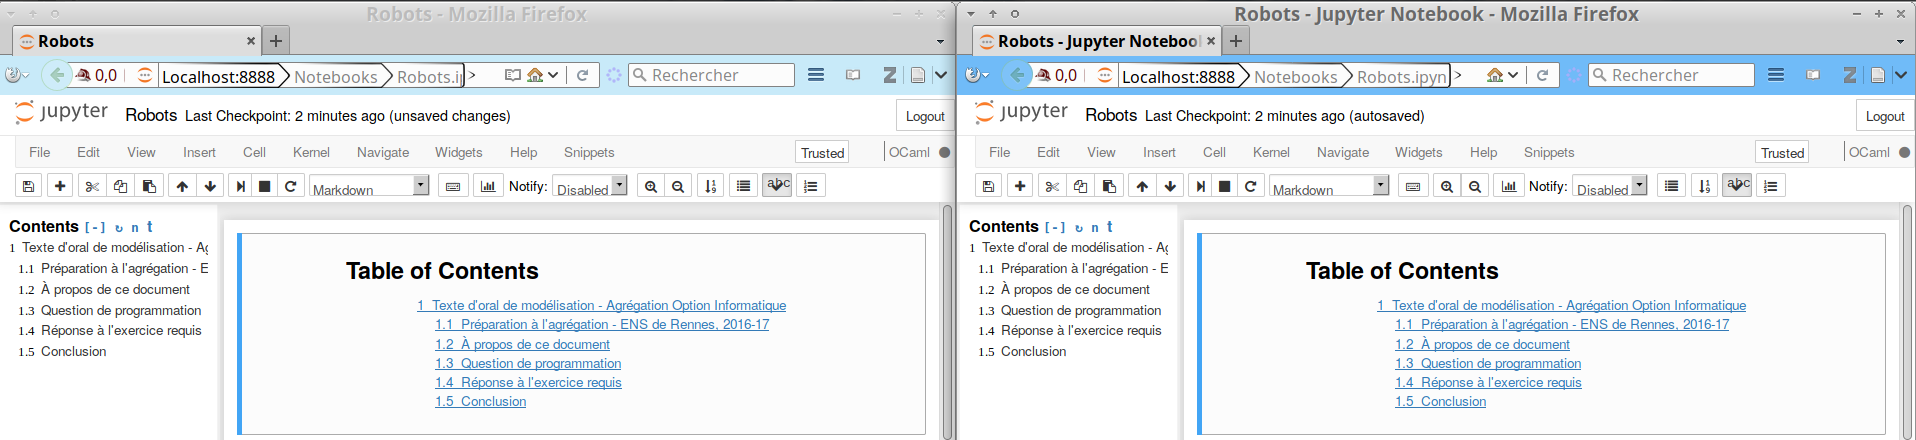
\includegraphics{editing_a_notebook.png}
\caption{Editing a notebook : before and after}
\end{figure}

\subsubsection{Home view : before and
after}\label{home-view-before-and-after}

\begin{figure}
\centering
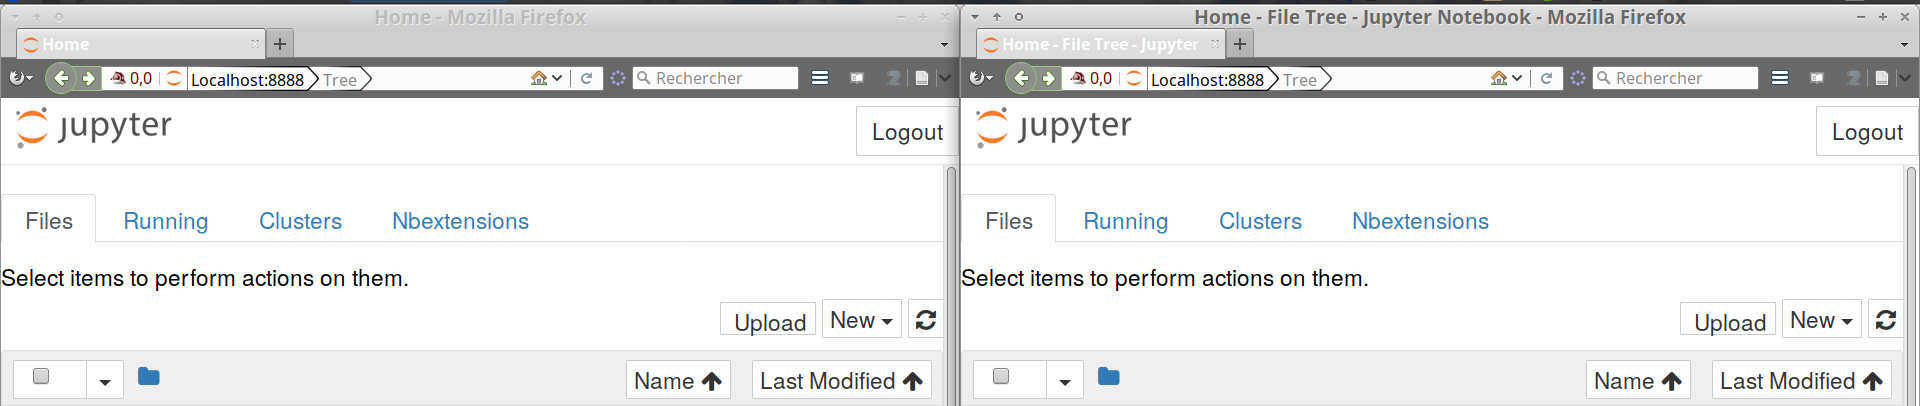
\includegraphics{home_view.png}
\caption{Home view : before and after}
\end{figure}

\begin{center}\rule{0.5\linewidth}{\linethickness}\end{center}

\subsection{Questions}\label{questions}

\subsubsection{\texorpdfstring{Bonus question : \emph{why would you want
to do \textbf{that}
?}}{Bonus question : why would you want to do that ?}}\label{bonus-question-why-would-you-want-to-do-that}

\begin{itemize}
\tightlist
\item
  Simple and honest answer : I am constantly using my
  \href{https://github.com/Naereen/uLogMe/}{uLogMe} software to watch
  and monitor the \emph{title} of the active window on my laptops, and I
  wanted to store the time spent editing Jupyter notebooks under a
  special category (``Notebooks'') and not under the general browsing
  time.
\item
  Fun answer : \ldots{} I am always curious about how a certain piece of
  software works, and I love tweaking ``just a little bit'' open-source
  pieces of code!
\end{itemize}

\subsubsection{\texorpdfstring{Interesting question : \emph{why writing
a tutorial and not a Jupyter Notebook extension (\texttt{nbextension})
?}}{Interesting question : why writing a tutorial and not a Jupyter Notebook extension (nbextension) ?}}\label{interesting-question-why-writing-a-tutorial-and-not-a-jupyter-notebook-extension-nbextension}

\begin{itemize}
\tightlist
\item
  Simple answer : I think (or though) it would be hard, as the changes
  explained below concern just a line or two in a few files, but on the
  core files of the software\ldots{}
\item
  Boring answer : I don't have time to produce a well-done nb extension,
  and maintain it\ldots{}
\end{itemize}

\begin{center}\rule{0.5\linewidth}{\linethickness}\end{center}

\subsection{License ?}\label{scroll-license}

\href{https://lbesson.mit-license.org/}{MIT Licensed} (file
\url{LICENSE}). © \href{https://GitHub.com/Naereen}{Lilian Besson},
2017.

\end{document}
